\documentclass[10pt,a4paper,twocolumn]{article}
\usepackage[T1]{fontenc}\usepackage{lmodern}
\usepackage[margin=1.8cm]{geometry}
\usepackage{graphicx,booktabs,amsmath,amssymb,xcolor,hyperref,microtype}
\usepackage[font=small]{caption}
\title{Constraints belong in the mixer: penalty vs.\ constraint-native QAOA\\ for cardinality-constrained portfolio selection on real market data}
\author{Francesco Pisaturo\\[2pt]
{\small ORCID: \href{https://orcid.org/0009-0002-5963-8036}{0009-0002-5963-8036}}\\[2pt]
{\small Independent work by a student; not an official publication of, nor endorsed by, any university.}\\[2pt]
{\small Code: \url{https://github.com/DevCisco/quantum-portfolio-selection}}}
\date{October 2026}
\hypersetup{colorlinks=true,linkcolor=blue!50!black,citecolor=blue!50!black,urlcolor=blue!50!black}
\begin{document}
\maketitle
\begin{abstract}
We compare two ways of handling the cardinality constraint $\sum_i x_i=k$ in QAOA for mean--variance portfolio selection: a quadratic penalty with the transverse-field mixer, and a constraint-native ring-XY mixer started from a Dicke state. Instead of a few synthetic instances we use 139 monthly instances built from rolling 12-month windows of 20 Euro Stoxx~50 constituents (2015--2026), with exact statevector simulation, exact optima by enumeration, bootstrap confidence intervals and paired Wilcoxon tests. Without noise, the constraint-native ansatz wins in 85--99\% of months. Its advantage over random guessing among feasible portfolios grows with problem size: the median ratio to the best penalty variant rises from $\approx 8\times$ at $n=8$ to $\approx 56\times$ at $n=16$. The result is robust to risk aversion, estimation window and a $64\times$ penalty scan. With several simultaneous group constraints, penalty QAOA falls below random guessing. Optimal parameters transfer between months at 12\% of the optimisation cost. Under an IBM Heron noise model the picture changes: Dicke-state preparation triples the two-qubit gate count, and the advantage survives only at depth $p=1$ with postselection. We make no claim of quantum advantage or of a tradeable strategy.
\end{abstract}

\section{Problem and methods}
For month $t$ we estimate annualised $\mu,\Sigma$ from the preceding 12 monthly log-returns (no look-ahead) and solve
\begin{equation}
\max_{x\in\{0,1\}^n}\ \mu^\top x-q\,x^\top\Sigma x\quad\text{s.t.}\ \textstyle\sum_i x_i=k,
\end{equation}
with $q=2$ unless stated. The objective is exactly a QUBO; only the constraint must be encoded. The cost is rescaled per month to $c\in[0,1]$ over the feasible set ($c=0$ at the optimum), so one parameter range serves every month. Prices are Yahoo Finance adjusted month-end closes; they are not redistributed.

\textbf{Ansätze.} \emph{Penalty}: $|+\rangle^{\otimes n}$, transverse mixer, $H=c+P(\sum_i x_i-k)^2$, with $P_\text{tight}$ (largest one-flip change of $c$, plus a margin) or $P_\text{auto}$ (the value chosen by qiskit-optimization's \texttt{LinearEqualityToPenalty}). \emph{Constraint-native}: ring XY mixer $\prod_{\langle ij\rangle}e^{-i\beta(X_iX_j+Y_iY_j)/2}$ in odd/even layers \cite{hadfield2019,wang2020}, started either from a computational-basis state with $k$ ones or from the Dicke state $|D_{n,k}\rangle$ \cite{bartschi2019}. For group constraints (exactly $k_g$ assets from group $g$) we use one XY ring per group and a product of per-group Dicke states.

\textbf{Protocol.} Exact statevector simulation; L-BFGS-B with 3--5 seeded random restarts. Metrics: $p_\text{opt}$, the probability of the exact optimum; $p_\text{feas}$; the approximation ratio conditional on feasibility; and the \emph{enhancement} $p_\text{opt}\cdot|\mathcal F|$, which is how many times better than a uniform guess among feasible portfolios. Enhancement can be compared across $n$; $p_\text{opt}$ cannot. Statistics: 5000-sample bootstrap CIs over months and paired Wilcoxon signed-rank tests.

\section{Results}
\textbf{Main comparison} ($n=12$, $k=4$, $p=2$, 139 months; Table~\ref{tab:main}). XY+Dicke has the highest $p_\text{opt}$ in 85\% (vs.\ $P_\text{tight}$) to 99\% (vs.\ XY with basis start) of months, Wilcoxon $p<10^{-14}$. With 100 shots it returns the exact optimum in 82\% of months, against 42\% for the best penalty variant. The basis start is almost as poor as the penalty despite being exactly feasible. This agrees with the alignment argument of He et al.\ \cite{he2023}: the mixer conserves the constraint, but the initial state must also spread over the feasible subspace.

\begin{table}[t]\centering\small
\caption{$n=12$, $k=4$, $p=2$, 139 months; means with 95\% bootstrap CIs.}\label{tab:main}
\begin{tabular}{lccc}\toprule
method & $p_\text{opt}$ & ratio$|$feas & $p_\text{feas}$\\\midrule
penalty $P_\text{tight}$ & .011 [.008,.014] & .647 & .501\\
XY, basis start & .007 [.000,.022] & .682 & 1\\
\textbf{XY, Dicke start} & \textbf{.035 [.030,.041]} & \textbf{.776} & 1\\
random feasible & .002 & .561 & --\\\bottomrule
\end{tabular}\end{table}

\textbf{Scaling} ($n=8\ldots16$, $k=\mathrm{round}(n/3)$, $p=1\ldots4$, 12 months per cell; Fig.~\ref{fig:scaling}). XY+Dicke enhancement grows from 10.5 at $n=8$ to 60.4 at $n=16$, and it improves monotonically with $p$. Penalty variants stay between 2 and 9 and are erratic in $p$. At $n=16$, $p=1$ they fall below random (0.5--0.6). The median ratio of enhancements, XY over the better penalty, rises from 7.9 to 55.9 (log-slope $+0.24$ per qubit). Each cell has only 12 months, so the claim is the trend, not any single cell.

\begin{figure*}[t]\centering
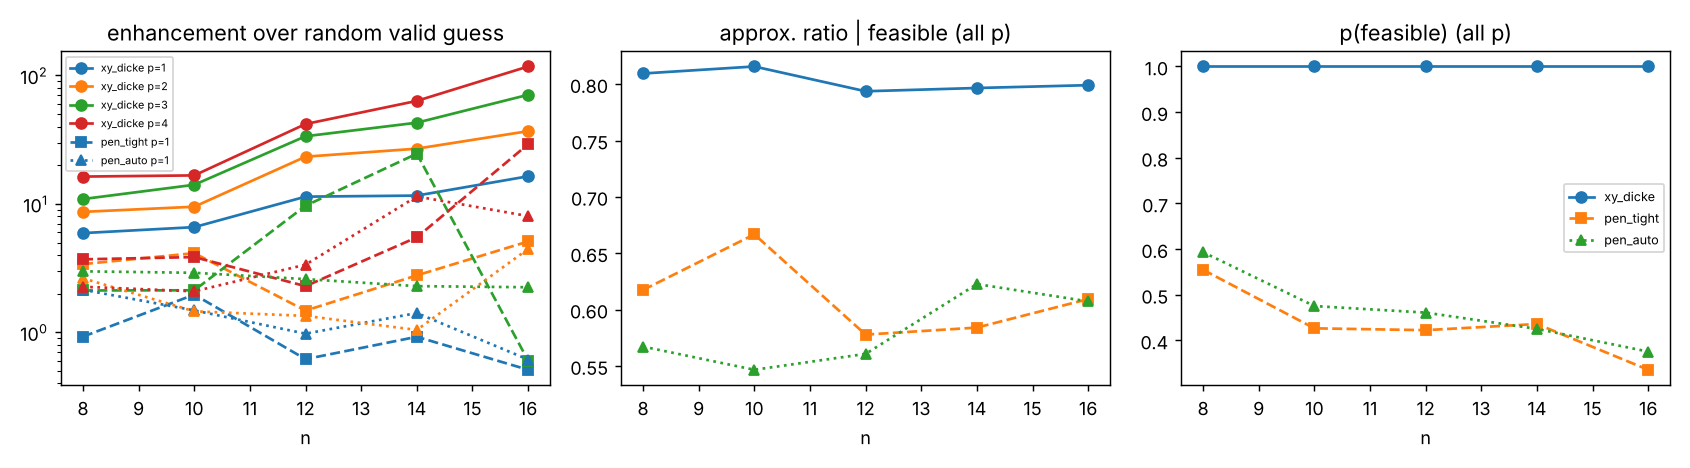
\includegraphics[width=.9\textwidth]{scaling.png}
\caption{Enhancement over random feasible guessing vs.\ $n$ and $p$ (left), conditional approximation ratio and $p_\text{feas}$ (centre, right).}\label{fig:scaling}\end{figure*}

\textbf{Robustness} ($n=12$, $p=2$, 46 months). Across $q\in\{0.5,2,8\}$ and windows of 6, 12 and 24 months, XY+Dicke beats both penalties in 74--91\% of months (all Wilcoxon $p\le2\cdot10^{-4}$). A scan of $P$ from $0.25$ to $16\times P_\text{tight}$ peaks at enhancement 5.1, against 16.6 for XY on the same months (Fig.~\ref{fig:pscan}). The automatic qiskit penalty ($\approx5.5\,P_\text{tight}$) gives 2.5. No penalty value closes the gap.

\begin{figure}[t]\centering
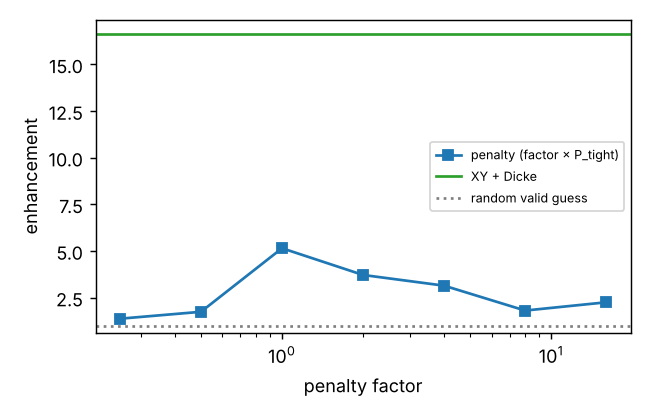
\includegraphics[width=.8\columnwidth]{penalty_scan.png}
\caption{Penalty scan at $n=12$, $p=2$.}\label{fig:pscan}\end{figure}

\textbf{Several constraints.} \emph{(a) Sectors}: exactly one IT, one industrial, one financial and one other stock (48 feasible portfolios). Grouped XY reaches $p_\text{opt}=0.262$ and finds the optimum in 100\% of months. The penalty reaches 0.009, \emph{below} the random-feasible 0.021, with $p_\text{feas}=0.17$. Grouped XY wins in every month ($p\approx10^{-24}$). A global XY ring that ignores sectors puts 89\% of its probability on portfolios that break the sector rule. \emph{(b) Mixed universe}: 8 stocks and 4 commodity futures in EUR, with 3 stocks and 1 commodity (224 feasible). Grouped XY reaches $p_\text{opt}=0.082$; the penalty reaches 0.012. XY is better in 92\% of months.

\textbf{Parameter transfer.} Re-optimising from the previous month's parameters with a single start gives the same $p_\text{opt}$ as five fresh restarts (0.035 vs.\ 0.035, Wilcoxon $p=0.40$) using 12\% of the cost function evaluations. Using last month's parameters with no re-optimisation loses almost nothing (0.034). So optimal QAOA parameters concentrate across market regimes.

\textbf{Hardware cost and noise.} We compiled both ansätze for an IBM Heron device model (FakeMarrakesh, heavy-hex, CZ gates; optimisation level 3, three transpiler seeds). The circuits were first verified against the simulator to $10^{-15}$. Both ansätze share the dense all-pairs ZZ cost layer. XY+Dicke needs $3.6\times$ the two-qubit gates at $p=1$ and $\approx2\times$ at $p=3$. The overhead is dominated by the one-off Dicke preparation, whose doubly controlled rotations are expensive on heavy-hex. In a noisy simulation ($n=8$, 11 months, parameters trained without noise, 8192 shots; Fig.~\ref{fig:noise}), XY loses exact feasibility ($p_\text{feas}\approx0.4$--0.55). Infeasible shots can be discarded at no cost (postselection on $\sum x=k$). After postselection, XY still leads at $p=1$ (4.6 vs.\ 3.8, better in 73\% of months). At $p=2$ its mean falls to 4.7 against 5.2 for the penalty, down from 9.3 without noise.

\begin{figure}[t]\centering
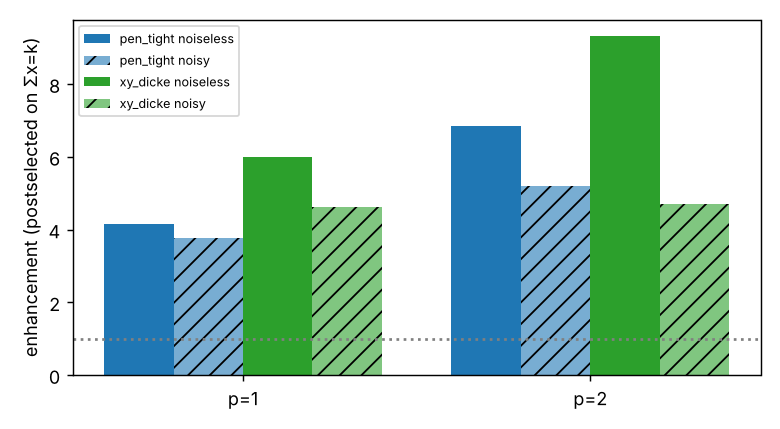
\includegraphics[width=.85\columnwidth]{noisy.png}
\caption{Postselected enhancement, noiseless vs.\ FakeMarrakesh noise, $n=8$.}\label{fig:noise}\end{figure}

\textbf{Out-of-sample (descriptive only).} Equal-weight holdings of the selected assets beat the Euro Stoxx~50 benchmark. So does an equal-weight portfolio of all 12 stocks, which shows that the effect comes from survivorship bias (today's constituents) and not from optimisation. In the mixed universe the penalty's portfolios even out-performed the exact optimum. Out-of-sample return therefore does not measure solver quality, and we do not report it as a result.

\section{Relation to prior work}
Constraint-preserving mixers were introduced by Hadfield et al.\ \cite{hadfield2019} and analysed for XY rings by Wang et al.\ \cite{wang2020}. Hodson et al.\ \cite{hodson2019} applied them to portfolio rebalancing on a small number of instances. Brandhofer et al.\ \cite{brandhofer2023} benchmarked penalty-based portfolio QAOA, including on IBM hardware. Surveys \cite{egger2020,herman2023} find no practical quantum advantage in finance to date. Our contributions are: (i) a paired statistical comparison over 139 real monthly instances of one market; (ii) evidence that the constraint-native advantage \emph{grows} with $n$ and survives every tuning of the penalty; (iii) the finding that multiple simultaneous constraints push penalty QAOA below random guessing; (iv) parameter transfer across months; (v) a compiled, noisy analysis that identifies Dicke-state preparation as the bottleneck on current hardware.

\section{Limitations and outlook}
Exact simulation limits us to $n\le16$. The scaling cells contain 12 months each. Depth is at most $p=4$, and the optimiser may under-train deep circuits, although it does so equally for all methods. The noise study uses one device model, $n=8$, and parameters that were not re-trained under noise. The financial setting is stylised: survivorship bias, no transaction costs, and front-month futures with roll effects. Natural next steps are cheaper or approximate Dicke preparation, layouts of the XY ring matched to the coupling map, error mitigation, MPS simulation beyond 16 qubits, and learned parameter initialisation that exploits the observed transfer.

\begin{thebibliography}{9}\footnotesize
\bibitem{hadfield2019} S.~Hadfield et al., ``From the quantum approximate optimization algorithm to a quantum alternating operator ansatz,'' \emph{Algorithms} 12, 34 (2019), arXiv:1709.03489.
\bibitem{wang2020} Z.~Wang, N.~Rubin, J.~Dominy, E.~Rieffel, ``XY mixers: analytical and numerical results for the quantum alternating operator ansatz,'' \emph{Phys.\ Rev.\ A} 101, 012320 (2020), arXiv:1904.09314.
\bibitem{bartschi2019} A.~B\"artschi, S.~Eidenbenz, ``Deterministic preparation of Dicke states,'' FCT 2019, arXiv:1904.07358.
\bibitem{hodson2019} M.~Hodson et al., ``Portfolio rebalancing experiments using the Quantum Alternating Operator Ansatz,'' arXiv:1911.05296 (2019).
\bibitem{brandhofer2023} S.~Brandhofer et al., ``Benchmarking the performance of portfolio optimization with QAOA,'' \emph{Quantum Inf.\ Process.} (2023), arXiv:2207.10555.
\bibitem{he2023} Z.~He et al., ``Alignment between initial state and mixer improves QAOA performance for constrained optimization,'' \emph{npj Quantum Inf.} (2023), arXiv:2305.03857.
\bibitem{egger2020} D.~J.~Egger et al., ``Quantum computing for finance: state-of-the-art and future prospects,'' \emph{IEEE Trans.\ Quantum Eng.} (2020), arXiv:2006.14510.
\bibitem{herman2023} D.~Herman et al., ``Quantum computing for finance,'' \emph{Nat.\ Rev.\ Phys.} (2023), arXiv:2201.02773.
\end{thebibliography}
\end{document}
